\section*{Summary of Scientific Discoveries}

\subsection*{Simulations of transport in nanostructured polymer membranes}
Our understanding of the microscopic structure of this type of LLC
membrane has greatly increased with the aid of simulations run using
Bridges. 

Equilibration simulations of greater than 500 nanoseconds yield
stable membrane configurations with the expected HII phase 
morphology. Various methods have been developed to characterize
the equilibrated system. Generally, all equilibrium properties are
compared to experimental measurements. We validated two methods
for measuring ionic conductivity from atomistic simulations. Both 
methods require long simulations (at least 500 ns) in order to give
accurate statistics. The distance between pores is an important
structural parameter which we have measured using atomic coordinates
and by simulating X-ray diffraction (XRD) experiments, a relatively
undeveloped technique in MD for periodic systems such as ours. We 
have been able to generate structures which match experimental pore
spacings within reason.

The X-ray diffraction simulations also give detailed information
about membrane structure on the angstrom lengthscale. Our simulations
have produced two dimensional X-ray diffraction patterns that 
contain all major features present in experimental studies. Producing
a matching pattern was not trivial and resulted in the discovery of
two metastable states. The two states are defined by the degree of 
local order inside the pore regions. The state which we had initially
studied is characterized by a disordered pore region, however the X-ray
diffraction pattern does not match experiment. We altered the starting 
configuration so that the benzene rings in the head group of each
monomer were stacked in a parallel displaced configuration relative
to each other. The resulting X-ray diffraction pattern of the new
configuration, after equilibration, is a much closer match to experiment.
Additionally, we were able to explain the spots that appear (red arrows
in Fig.~\ref{metastable}) contrary to how it was originally reported. The spots 
were assumed to be caused by the 40 degree tilt angle of the alkyl
tails with respect to the plane of each stacked monomer layer, a 
common feature of liquid crystal systems. However, we were able to 
produce the same spots using configurations with an average tilt angle
close to zero. Our most impactful finding remains as the discovery of 
two metastable states. This will be the subject of a publication which 
will be submitted in the coming months. In the future, we will conduct
free energy calculations that will quantify the relative stability of
the two states and and help predict what experimental conditions might
lead to each. We will also explore transport properties in each 
configuration to see which state provides optimal performance. 

\begin{figure}
\caption{}
\label{figure:metastable}
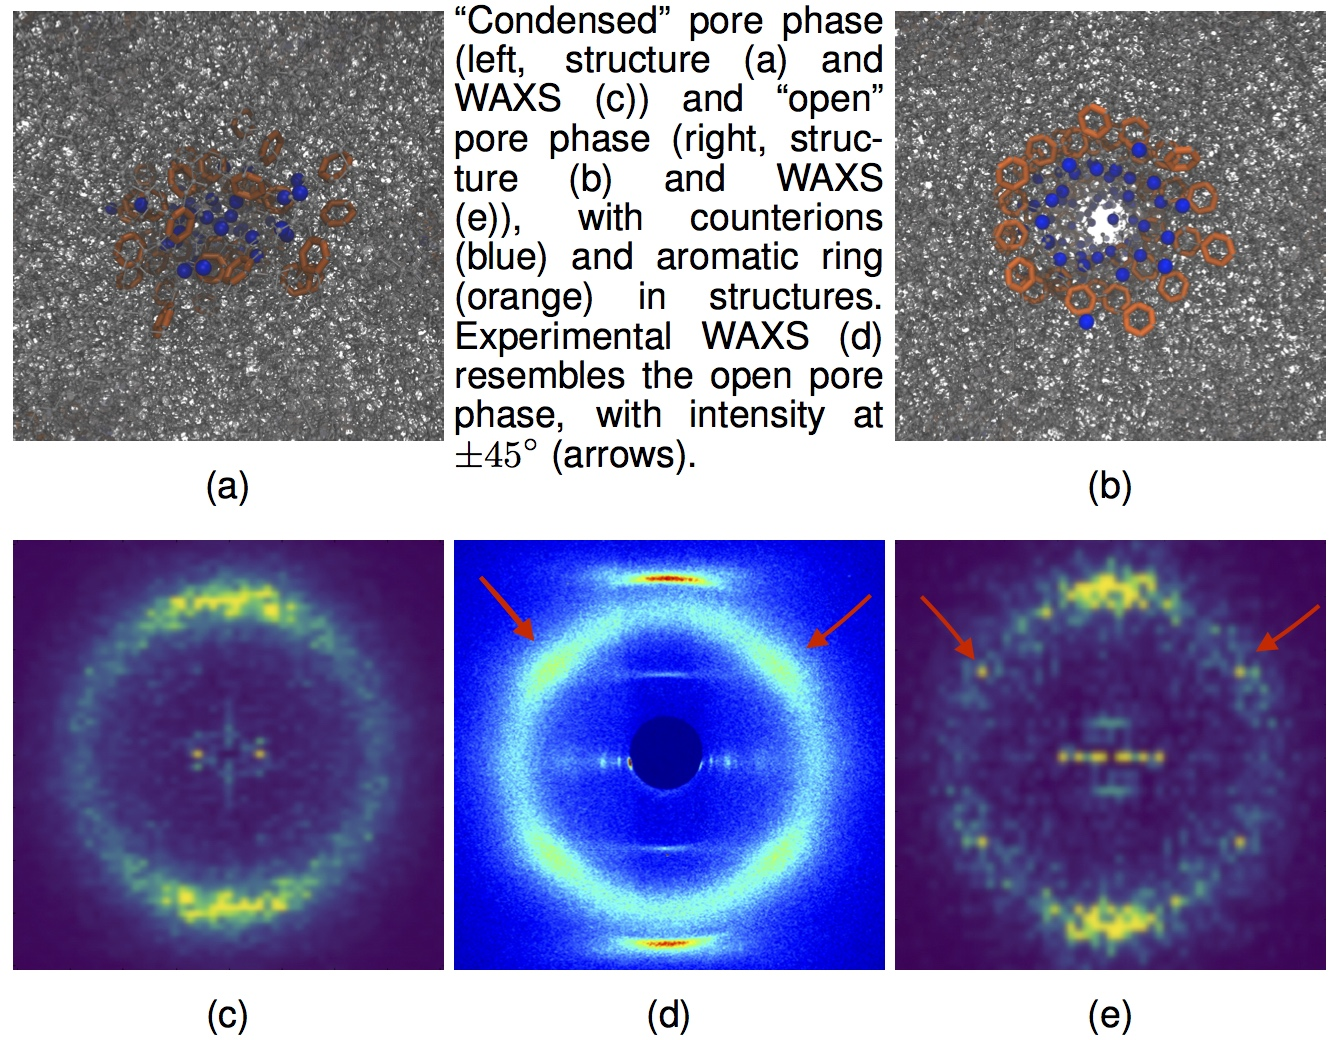
\includegraphics[width=.9\textwidth]{porestructures.jpg}
\centering
\end{figure}

The next step for our system is to solvate it with water. In parallel 
to the preceding work, we have worked to develop methods which will be
used to study the solvated system. While measuring ionic conductivity 
and running XRD simulations will work just the same, equilibration is 
non-trivial. We do not know exactly the equilibrium content of water 
or where the water is situated in the membrane. While it is clear that 
most water should be in the hydrophilic pore region, simulations have shown that an 
appreciable amount of water can exist in the tail region near the 
slightly hydrophilic ester group. The best way to figure out how much 
water should be in the pore is to run very long equilibration simulations
and allow the simulations to tell us. Our current approach is to create
water baths at each face of the membrane and allow water to diffuse into
the membrane. We have learned that we can equilibrate a membrane with
water in 1000 nanoseconds. Studies of the hydrated, 'lyotropic', phase
will be the subject of a future publication.
